\section{Matlab}
In order to aid the design of the algorithms Matlab models were produced and
tested.

\subsection{Correlation}

Two music files were used for testing.
These were chosen because they featured a range of different sounds, covering a large range of the human hearing spectrum, and of various intensities.
The two pieces of music were significantly different styles to introduce more variance.
A lag was produced between these two and then they were mixed together.
The cross correlation was taken between one of them and the mix of the two, the result of which can be seen in figure \ref{fig:modelcrosscorr}.
The distinct peak at 23 samples was detected, the shift applied, and the inverse of the respective sample then added to the mix.
This cleared up the audio allowing the second, original, unmixed audio signal to be heard.
When the two signals were mixed, if the amplitude of the mixed signals was different to that of the noise input, over-cancellation would occur and, although reduced, the noise signal could still be heard over the cancelled signal.

\begin{figure}[H]
	\centering
	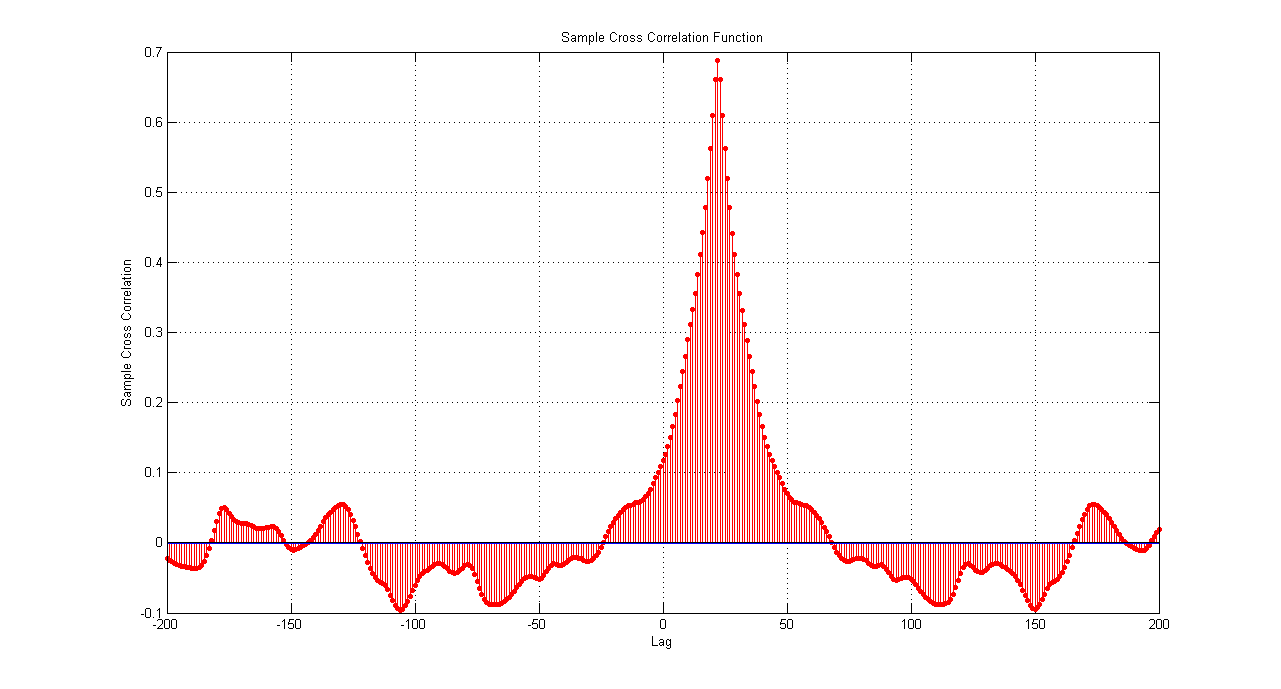
\includegraphics[width=\textwidth]{./img/crosscorr.png}
	\caption{Cross correlation of two signals}
	\label{fig:modelcrosscorr}
\end{figure}

\subsection{LMS}
The LMS algorithm was modelled in two ways.
Firstly an inbuilt toolbox of Matlab was used, in order to provide a model to test this projects code against.
This filter successfully cancelled out one signal from another, as can be seen in figure \ref{fig:modellmscancel}.
For this test a simple sine wave was generated and used as both the noise and the heard signals.
The LMS filter length being set at 50.
The output shown is the result of virtual feedback, and represents what would be actually reaching the users ear.

\begin{figure}[H]
	\centering
	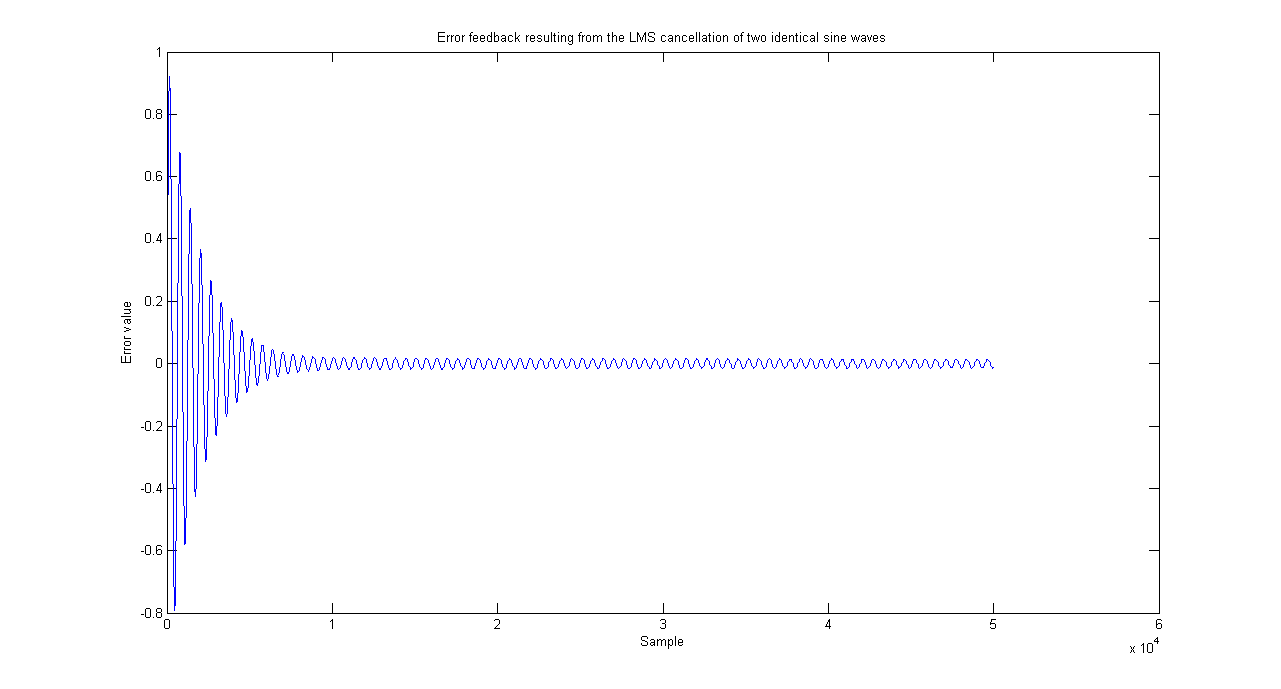
\includegraphics[width=\textwidth]{./img/lmssnr_cancel.png}
	\caption{LMS error feedback for identical noise and heard inputs, using Matlabs DSP toolbox}
	\label{fig:modellmscancel}
\end{figure}

\noindent As both the noise and heard signals being used are identical then the ideal error value would be zero.
However the cancellation achieved is acceptably significant, and would notably improve the users audio experience.
\\
\\
LMS filters can be of range of lengths, however some will produce a better cancellation signal.
The two music files were used, and filtered at various filter lengths in order to determine the optimal filter length.
Figure \ref{fig:modellmsfiltlen} shows the peak SNR values of the error feedback signal, and clearly shows that optimal cancellation can be achieved with a filter length of 50.

\begin{figure}[H]
	\centering
	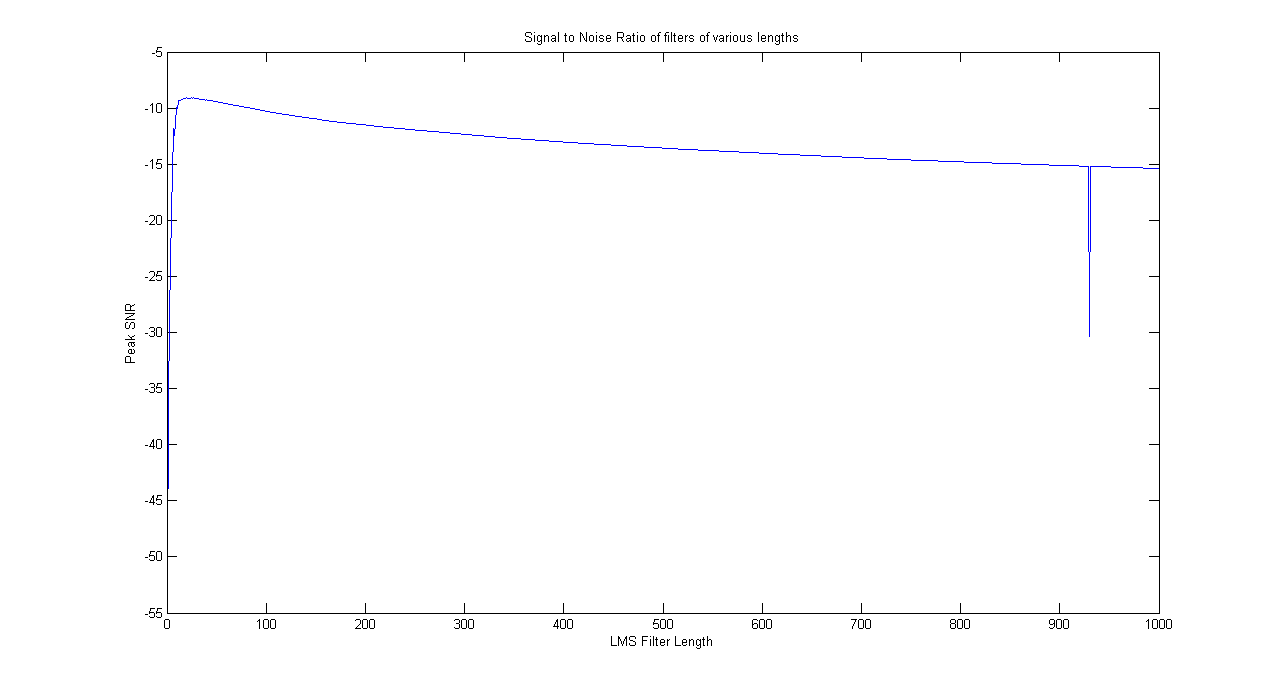
\includegraphics[width=\textwidth]{./img/lmssnr_graph.png}
	\caption{LMS filter length against signal to noise ratio}
	\label{fig:modellmsfiltlen}
\end{figure}

\noindent The second model produced was using a structure that was more compatible with how it would be implemented on the DSP.
The advantage of this method was that the DSP code could be very easily produced based off the Matlab code, while still allowing it to be checked against the model.
Given the same inputs, this model works about on par with the one provided by Matlab (figure \ref{fig:modellmscancelmine}), however taking longer to close onto the optimal values.

\begin{figure}[H]
	\centering
	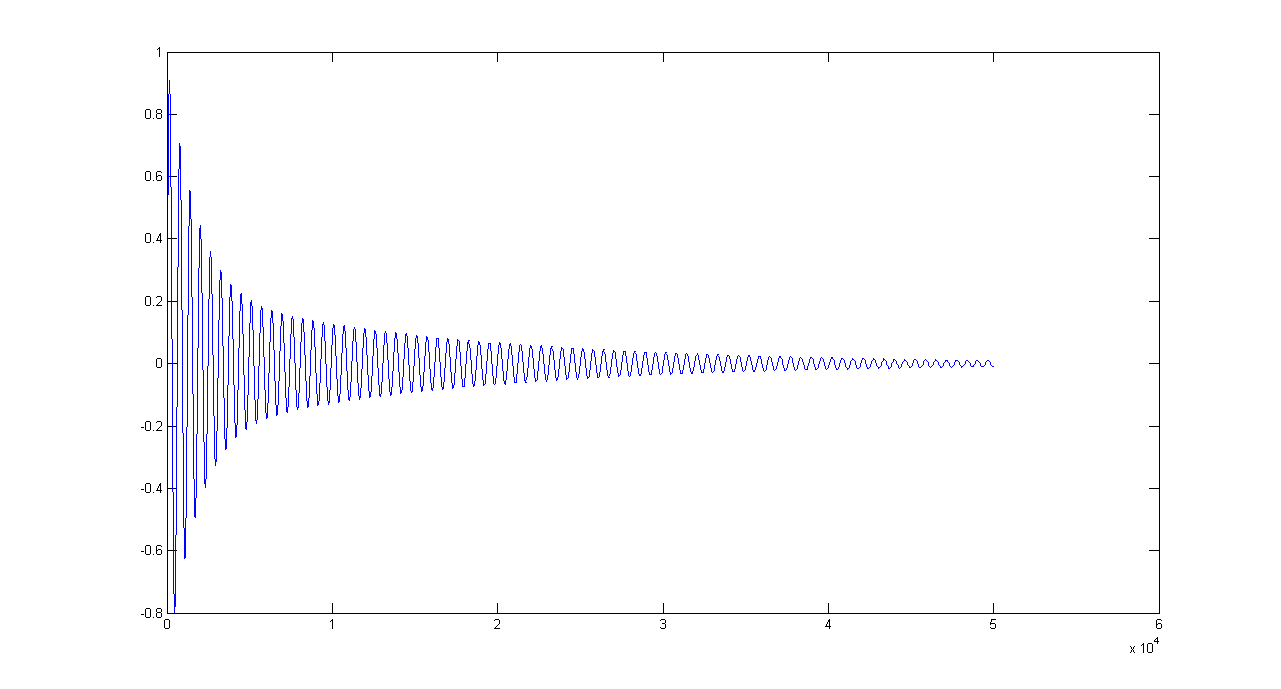
\includegraphics[width=\textwidth]{./img/lmssnr_cancel_mine.png}
	\caption{LMS error feedback for identical noise and head inputs, using the code written for this project}
	\label{fig:modellmscancelmine}
\end{figure}

